\chapter{Congruences and Modular Arithmetic}

\section{Congruence}

\begin{definition}
Let $m \in \N$. Integers $a$ and $b$ are \emph{congruent modulo $m$}, written
$a \equiv b \Mod{m}$, if $m \mid (a - b)$.
\end{definition}

\begin{example}
$17 \equiv 2 \Mod 5$ since $5 \mid 15$; $-3 \equiv 9 \Mod 4$ since $4 \mid -12$;
$10 \not\equiv 3 \Mod 4$ since $4\nmid 7$. $a\equiv 0 \Mod m$ means $m \mid a$.
\end{example}

\begin{proposition}[Congruence is an Equivalence Relation, CER]
For all $a,b,c\in\Z$:
\begin{enumerate}
  \item (reflexive) $a \equiv a \Mod m$;
  \item (symmetric) $a \equiv b \Rightarrow b \equiv a \Mod m$;
  \item (transitive) $a \equiv b$ and $b \equiv c$ $\Rightarrow a \equiv c \Mod m$.
\end{enumerate}
\end{proposition}
\begin{proof}
(1) $m \mid 0$. (2) If $m \mid a - b$ then $m \mid -(a-b) = b - a$. (3) $m \mid (a - b) + (b - c)
= a - c$ by DIC.
\end{proof}

\begin{theorem}[Congruence Add and Multiply, CAM]
If $a \equiv a'$ and $b \equiv b' \Mod m$, then
\[ a + b \equiv a' + b', \qquad a - b \equiv a' - b', \qquad ab \equiv a'b' \Mod m. \]
Consequently $a^k \equiv (a')^k \Mod m$ for every $k \in \N$ (Congruence Power, CP).
\end{theorem}
\begin{proof}
For products: $ab - a'b' = a(b - b') + b'(a - a')$, and $m$ divides both terms, so DIC applies.
The power rule follows by induction on $k$.
\end{proof}

\begin{important}[Division is not automatic]
We can add, subtract, multiply and take powers, but \emph{not} divide freely:
$2\cdot 3 \equiv 2 \cdot 8 \Mod{10}$ but $3 \not\equiv 8 \Mod {10}$.
\end{important}

\begin{proposition}[Congruence Divide, CD]
If $ac \equiv bc \Mod m$ and $\gcd(c,m) = 1$, then $a \equiv b \Mod m$.
\end{proposition}
\begin{proof}
$m \mid c(a - b)$ and $\gcd(m,c) = 1$, so by CAD $m \mid a - b$.
\end{proof}

\begin{proposition}[Congruent iff Same Remainder, CISR]
$a \equiv b \Mod m$ if and only if $a$ and $b$ leave the same remainder on division by $m$.
\end{proposition}
\begin{proof}
Write $a = q_1m + r_1$, $b = q_2m + r_2$ with $0 \le r_i < m$. Then
$a - b = (q_1 - q_2)m + (r_1 - r_2)$, so $m \mid a - b \iff m \mid r_1 - r_2$, and since
$\abs{r_1 - r_2} < m$, this happens iff $r_1 = r_2$.
\end{proof}

\section{Computing with congruences}

\begin{example}
Find the remainder when $2^{100}$ is divided by $7$. Since $2^3 = 8 \equiv 1 \Mod 7$,
\[ 2^{100} = 2^{99}\cdot 2 = (2^3)^{33}\cdot 2 \equiv 1^{33}\cdot 2 = 2 \Mod 7. \]
The remainder is $2$.
\end{example}

Powers of $2$ modulo $7$ go round a cycle of length $3$, which is why only $100 \bmod 3$
matters:
\begin{center}
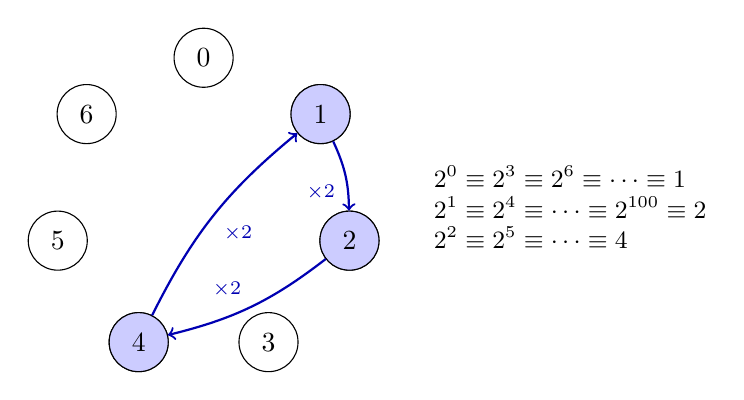
\begin{tikzpicture}
  \foreach \k in {0,...,6} {
    \node[draw,circle,minimum size=0.75cm,inner sep=0pt] (r\k) at ({90-360/7*\k}:1.9) {$\k$};
  }
  \foreach \k in {1,2,4} { \node[draw,circle,minimum size=0.75cm,inner sep=0pt,fill=blue!20] at ({90-360/7*\k}:1.9) {$\k$}; }
  \draw[->,thick,blue!70!black] (r1) to[bend left=12] node[auto,swap,font=\scriptsize] {$\times 2$} (r2);
  \draw[->,thick,blue!70!black] (r2) to[bend left=12] node[auto,swap,font=\scriptsize] {$\times 2$} (r4);
  \draw[->,thick,blue!70!black] (r4) to[bend left=12] node[auto,swap,font=\scriptsize] {$\times 2$} (r1);
  \node[align=left,font=\small,right] at (2.8,0) {$2^0 \equiv 2^3 \equiv 2^6 \equiv \cdots \equiv 1$\\
    $2^1 \equiv 2^4 \equiv \cdots \equiv 2^{100} \equiv 2$\\ $2^2 \equiv 2^5 \equiv \cdots \equiv 4$};
\end{tikzpicture}
\end{center}

\begin{example}
Find the last digit of $7^{2022}$ (i.e.\ the remainder mod $10$). $7^2 = 49 \equiv -1 \Mod{10}$,
so $7^4 \equiv 1$. Then $7^{2022} = (7^4)^{505}\cdot 7^2 \equiv 49 \equiv 9 \Mod{10}$. Last
digit: $9$.
\end{example}

\begin{example}[Repeated squaring]
Compute $3^{45} \bmod 23$. Squaring: $3^1 = 3$, $3^2 = 9$, $3^4 = 81 \equiv 12$,
$3^8 \equiv 144 \equiv 6$, $3^{16} \equiv 36 \equiv 13$, $3^{32} \equiv 169 \equiv 8 \Mod{23}$.
With $45 = 32 + 8 + 4 + 1$:
\[ 3^{45} \equiv 8 \cdot 6 \cdot 12 \cdot 3 = 1728 \equiv 1728 - 75\cdot 23 = 1728 - 1725 = 3
\Mod{23}. \]
(Consistent with $3^{11} \equiv 1 \Mod{23}$, since then $3^{45} = (3^{11})^4\cdot 3\equiv 3$.)
\end{example}

\begin{example}[Divisibility by 9 and 11]
Write $n = \sum_{i=0}^k d_i 10^i$. Since $10 \equiv 1 \Mod 9$, $n \equiv \sum d_i \Mod 9$.
Since $10 \equiv -1 \Mod{11}$, $n \equiv \sum (-1)^i d_i \Mod{11}$. For example
$918082$: digit sum $28 \equiv 1 \Mod 9$, so $9 \nmid 918082$; alternating sum from the right
$2 - 8 + 0 - 8 + 1 - 9 = -22 \equiv 0 \Mod{11}$, so $11 \mid 918082$.
\end{example}

\begin{example}
Show $x^2 \equiv 3 \Mod 4$ has no solutions (hence $x^2 + y^2 = 4k + 3$ is impossible).
Every $x$ is congruent to $0,1,2,3$ mod $4$, and then $x^2 \equiv 0,1,0,1$. Never $3$.
\end{example}

\section{Congruence classes and $\Z_m$}

\begin{definition}
The \emph{congruence class} of $a$ modulo $m$ is $\cls{a} = \{x \in \Z : x \equiv a \Mod m\}
= \{a + km : k \in \Z\}$. The set of classes is
$\Zm{m} = \{\cls 0, \cls 1, \dots, \cls{m-1}\}$, with operations
$\cls a + \cls b = \cls{a+b}$ and $\cls a \cdot \cls b = \cls{ab}$.
\end{definition}

By CAM these operations are well defined (independent of the representatives chosen), and by
CISR the $m$ listed classes are distinct and cover $\Z$. $\Zm m$ satisfies the usual rules of
arithmetic (commutative, associative, distributive, identities $\cls 0$ and $\cls 1$, additive
inverses $-\cls a = \cls{-a}$).

For $m = 5$, wrapping the integer line around a circle of circumference $5$ puts each class
on one spoke:
\begin{center}
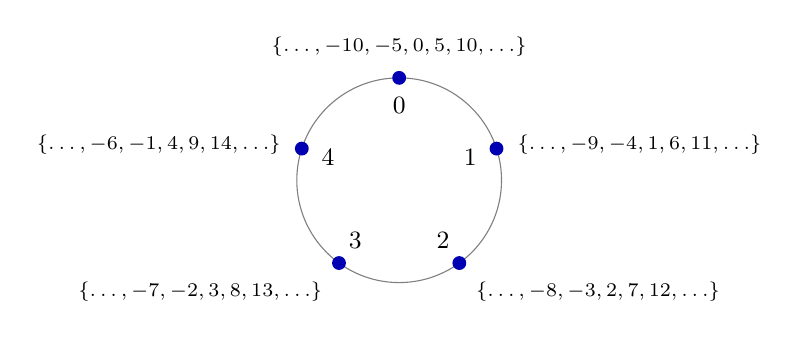
\begin{tikzpicture}
  \draw[gray] (0,0) circle (1.3);
  \foreach \k/\an/\lab in {0/south/{\dots,-10,-5,0,5,10,\dots},1/west/{\dots,-9,-4,1,6,11,\dots},2/north west/{\dots,-8,-3,2,7,12,\dots},3/north east/{\dots,-7,-2,3,8,13,\dots},4/east/{\dots,-6,-1,4,9,14,\dots}} {
    \fill[blue!70!black] ({90-72*\k}:1.3) circle (2.5pt);
    \node at ({90-72*\k}:0.95) {\small $\cls{\k}$};
    \node[font=\scriptsize,anchor=\an] at ({90-72*\k}:1.45) {$\{\lab\}$};
  }
\end{tikzpicture}
\end{center}

\begin{example}[Multiplication table of $\Zm 6$, non-zero part]
\begin{center}
\begin{tabular}{c|ccccc}
$\cdot$ & $1$ & $2$ & $3$ & $4$ & $5$\\
\hline
$1$ & $1$ & $2$ & $3$ & $4$ & $5$\\
$2$ & $2$ & $4$ & $0$ & $2$ & $4$\\
$3$ & $3$ & $0$ & $3$ & $0$ & $3$\\
$4$ & $4$ & $2$ & $0$ & $4$ & $2$\\
$5$ & $5$ & $4$ & $3$ & $2$ & $1$\\
\end{tabular}
\end{center}
Note $\cls 2\cls 3 = \cls 0$: $\Zm 6$ has zero divisors, and only $\cls 1, \cls 5$ have
multiplicative inverses.
\end{example}

\section{Inverses in $\Zm m$}

\begin{definition}
$\cls b$ is a \emph{multiplicative inverse} of $\cls a$ in $\Zm m$ if $\cls a\cls b = \cls 1$,
i.e.\ $ab \equiv 1 \Mod m$.
\end{definition}

\begin{theorem}[Inverses in $\Zm m$, INV $\Zm m$]
$\cls a$ has a multiplicative inverse in $\Zm m$ if and only if $\gcd(a,m) = 1$, and then the
inverse is unique. In particular, if $p$ is prime, every non-zero element of $\Zm p$ has an
inverse ($\Zm p$ is a field).
\end{theorem}
\begin{proof}
$ab \equiv 1 \Mod m \iff ab + mk = 1$ for some $k \iff \gcd(a,m) = 1$ (CCT). Uniqueness: if
$ab \equiv ab' \equiv 1$, then multiplying $ab \equiv ab'$ by $b$ gives $b \equiv b'$.
\end{proof}

\begin{example}
Find $\cls{17}^{-1}$ in $\Zm{37}$. EEA on $37$ and $17$: $37 = 2\cdot 17 + 3$, $17 = 5\cdot 3 + 2$,
$3 = 1\cdot 2 + 1$.
\begin{center}
\begin{tabular}{rrrr}
\toprule
$x$ & $y$ & $r$ & $q$\\
\midrule
$1$ & $0$ & $37$ & \\
$0$ & $1$ & $17$ & \\
$1$ & $-2$ & $3$ & $2$\\
$-5$ & $11$ & $2$ & $5$\\
$6$ & $-13$ & $1$ & $1$\\
\bottomrule
\end{tabular}
\end{center}
So $37(6) + 17(-13) = 1$, giving $17 \cdot (-13) \equiv 1 \Mod{37}$. Thus
$\cls{17}^{-1} = \cls{-13} = \cls{24}$. Check: $17\cdot 24 = 408 = 11\cdot 37 + 1$.
\end{example}

\section{Linear congruences}

\begin{theorem}[Linear Congruence Theorem, LCT]
Let $d = \gcd(a,m)$. The congruence $ax \equiv c \Mod m$ has a solution if and only if
$d \mid c$. In that case, if $x_0$ is one solution, the complete solution is
\[ x \equiv x_0 \Mod{\tfrac md}, \]
equivalently $x \equiv x_0,\ x_0 + \tfrac md,\ \dots,\ x_0 + (d-1)\tfrac md \Mod m$, which are
$d$ distinct classes mod $m$.
\end{theorem}
\begin{proof}
$ax \equiv c \Mod m \iff ax + my = c$ for some $y \in \Z$. Apply LDET 1 and LDET 2: the $x$-values of
solutions are exactly $x_0 + \frac md n$, $n \in \Z$.
\end{proof}

\begin{example}
Solve $17x \equiv 5 \Mod{37}$. Since $\gcd = 1$, multiply by the inverse $24$:
$x \equiv 24\cdot 5 = 120 \equiv 120 - 111 = 9 \Mod{37}$. Check: $17 \cdot 9 = 153 = 4\cdot 37 + 5$.
\end{example}

\begin{example}
Solve $14x \equiv 10 \Mod{40}$. Here $d = \gcd(14,40) = 2$ and $2 \mid 10$, so there are
solutions. Divide everything by $2$: $7x \equiv 5 \Mod{20}$. Since $7\cdot 3 = 21 \equiv 1$,
$7^{-1} \equiv 3$ and $x \equiv 15 \Mod{20}$. As classes mod $40$: $x \equiv 15$ or
$35 \Mod{40}$. Check: $14\cdot 15 = 210 = 5\cdot 40 + 10$ and $14 \cdot 35 = 490 = 12\cdot 40 + 10$.
\end{example}

\begin{example}
$6x \equiv 4 \Mod 9$ has no solution, since $\gcd(6,9) = 3 \nmid 4$.
\end{example}

\begin{important}[Dividing a congruence]
When you divide $ax \equiv c \Mod m$ by $d = \gcd(a,m)$, you must divide the modulus as well:
$ax \equiv c \Mod m \iff \frac ad x \equiv \frac cd \Mod{\frac md}$.
\end{important}

\section{Common pitfalls}
\begin{itemize}
  \item Cancelling a factor that is not coprime to $m$.
  \item Forgetting that negative representatives are allowed and often convenient
        ($7^2 \equiv -1 \Mod{10}$).
  \item Reducing exponents modulo $m$: $a^k \not\equiv a^{k \bmod m}$ in general. (Exponents
        reduce modulo $p-1$ via Fermat, Chapter 9.)
  \item Giving the solution of a linear congruence only mod $m/d$ when asked for classes mod $m$,
        or vice versa.
\end{itemize}

\section{Summary}
\begin{itemize}
  \item $a\equiv b \Mod m \iff m \mid a - b \iff$ same remainder mod $m$.
  \item CAM/CP: congruences may be added, subtracted, multiplied, raised to powers; division only
        by numbers coprime to $m$ (CD).
  \item $\Zm m$ is the set of classes; $\cls a$ is invertible iff $\gcd(a,m) = 1$; find inverses
        with the EEA.
  \item LCT: $ax \equiv c \Mod m$ is solvable iff $d = \gcd(a,m) \mid c$, with a unique solution
        mod $m/d$ ($d$ solutions mod $m$).
\end{itemize}
